%% This is file `elsarticle-template-1-num.tex',
%%
%% Copyright 2009 Elsevier Ltd
%%
%% This file is part of the 'Elsarticle Bundle'.
%% ---------------------------------------------
%%
%% It may be distributed under the conditions of the LaTeX Project Public
%% License, either version 1.2 of this license or (at your option) any
%% later version.  The latest version of this license is in
%%    http://www.latex-project.org/lppl.txt
%% and version 1.2 or later is part of all distributions of LaTeX
%% version 1999/12/01 or later.
%%
%% Template article for Elsevier's document class `elsarticle'
%% with numbered style bibliographic references
%%
%% $Id: elsarticle-template-1-num.tex 149 2009-10-08 05:01:15Z rishi $
%% $URL: http://lenova.river-valley.com/svn/elsbst/trunk/elsarticle-template-1-num.tex $
%%
\documentclass[final,12pt]{elsarticle}
\usepackage{geometry}
\geometry{left=1.9cm, top=1.9cm, right=1.9cm, bottom=1.9cm, footskip=0.5cm}

%% Use the option review to obtain double line spacing
%% \documentclass[preprint,review,12pt]{elsarticle}

%% Use the options 1p,twocolumn; 3p; 3p,twocolumn; 5p; or 5p,twocolumn
%% for a journal layout:
%% \documentclass[final,1p,times]{elsarticle}
%% \documentclass[final,1p,times,twocolumn]{elsarticle}
%% \documentclass[final,3p,times]{elsarticle}
%% \documentclass[final,3p,times,twocolumn]{elsarticle}
%% \documentclass[final,5p,times]{elsarticle}
%% \documentclass[final,5p,times,twocolumn]{elsarticle}

%% The graphicx package provides the includegraphics command.
\usepackage{graphicx}
%% The amssymb package provides various useful mathematical symbols
\usepackage{amssymb}
%% The amsthm package provides extended theorem environments
%% \usepackage{amsthm}


%% natbib.sty is loaded by default. However, natbib options can be
%% provided with \biboptions{...} command. Following options are
%% valid:

%%   round  -  round parentheses are used (default)
%%   square -  square brackets are used   [option]
%%   curly  -  curly braces are used      {option}
%%   angle  -  angle brackets are used    <option>
%%   semicolon  -  multiple citations separated by semi-colon
%%   colon  - same as semicolon, an earlier confusion
%%   comma  -  separated by comma
%%   numbers-  selects numerical citations
%%   super  -  numerical citations as superscripts
%%   sort   -  sorts multiple citations according to order in ref. list
%%   sort&compress   -  like sort, but also compresses numerical citations
%%   compress - compresses without sorting
%%
%% \biboptions{comma,round}

% \biboptions{}

\journal{JP Morgan QR Technical Screening}

\begin{document}

\begin{frontmatter}

%% Title, authors and addresses

\title{User Guides: FRED Data Download Application}

%% use the tnoteref command within \title for footnotes;
%% use the tnotetext command for the associated footnote;
%% use the fnref command within \author or \address for footnotes;
%% use the fntext command for the associated footnote;
%% use the corref command within \author for corresponding author footnotes;
%% use the cortext command for the associated footnote;
%% use the ead command for the email address,
%% and the form \ead[url] for the home page:
%%
%% \title{Title\tnoteref{label1}}
%% \tnotetext[label1]{}
%% \author{Name\corref{cor1}\fnref{label2}}
%% \ead{email address}
%% \ead[url]{home page}
%% \fntext[label2]{}
%% \cortext[cor1]{}
%% \address{Address\fnref{label3}}
%% \fntext[label3]{}


%% use optional labels to link authors explicitly to addresses:
%% \author[label1,label2]{<author name>}
%% \address[label1]{<address>}
%% \address[label2]{<address>}

\author{Johnew Zhang}

%\address{}

\begin{abstract}
In this document, we will walk through how to use the FRED data downloader application.
\end{abstract}

%\begin{keyword}
%Science \sep Publication \sep Complicated

%\end{keyword}

\end{frontmatter}

%%
%% Start line numbering here if you want
%%
%\linenumbers

%% main text
\section{Prerequisites}
\begin{description}
\item[System Requirement] Windows/MacOS (This application has only been tested on MacOS)
\item[Programming Environment] Python 2.7+ (Recommended to install through Anaconda) 
\item[Library Requirement] pandas, requests, json, Tk (please visit http://www.tkdocs.com/tutorial/install.html for installation instruction)
\item[Internet] Good internet connection. (Warning: It may be constraint by company's internet proxy)
\end{description}

\section{Walk-Through}
\subsection{Run Application}
Assume we have downloaded the FredAPI.zip file, now we can open either your command line or terminal to direct to the unzipped FredAPI folder. Then type
\begin{verbatim}
$ python main.py
\end{verbatim}
or check Figure 1 
\begin{figure}[h]
\centering
\includegraphics[width=0.6\linewidth]{img/first_step.png}
\caption{First Step}
\end{figure}

Then a pop-up window will open as the one in Figure 2. 

\begin{figure}[h]
\centering
\includegraphics[width=0.6\linewidth]{img/search_page.png}
\caption{Search Page}
\end{figure}

\newpage

\subsection{Search Page}
Now we have opened the FRED Data Downloader application so let's do some search. in the search phase, we can see three elements, a QUIT button, a search TextBox and a Search Button. 
\begin{description}
\item[QUIT Button] Click to quit the application.
\item[Search TextBox] Input our key words. We can press ENTER to start the data query.
\item[Search Button] Search Button. We can click this to start the data query.
\end{description}

\subsection{Query Result}
After we've pressed ENTER or Search Button, we may need to wait a bit to see the search result. If the search is successful, we will see the result as in Figure 3. In Figure 3., we searched "US GDP" and the FRED GDPC1 shows up as the top search result. When there is no search result, the page will simply return ``No data related to the search key words!".
\begin{figure}[h]
\centering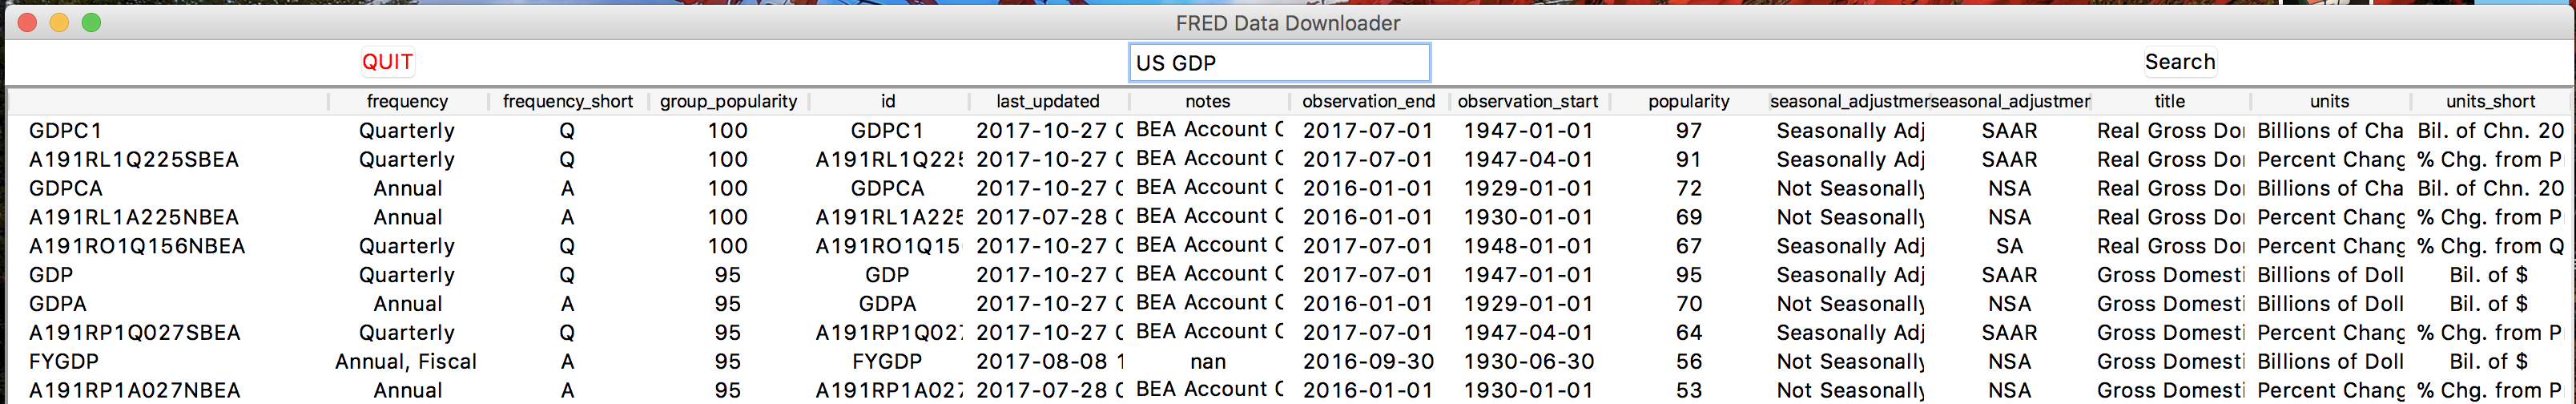
\includegraphics[width=1\linewidth]{img/query_result.png}
\caption{Query Result Page}
\end{figure}

\subsection{Download Data}
We've obtained our search result so how can we download the data? It is simple. We just need to double click the data we are interested in the list and then a download section will show up below the query table. It is shown as in Figure 4.

\begin{figure}[h]
\centering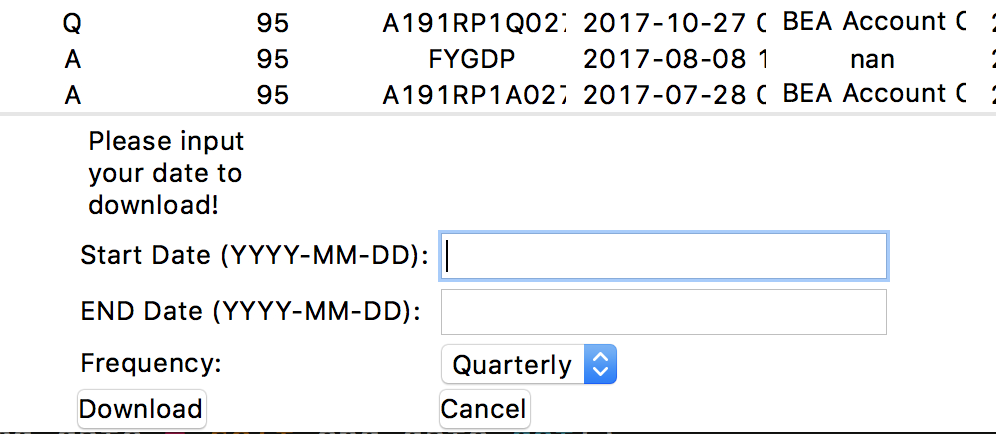
\includegraphics[width=0.5\linewidth]{img/download_page.png}
\caption{Download Page}
\end{figure}

We can specify the start data, end data and frequency of our data here. Next we can click ``Download" to get the data and save it on our local drive. Figure 5 shows the save as dialog after we clicked ``Download" and we need to provide a file name for the application to save the data we are interested. If we made a mistake in our input, a Error dialog will show up to let us know. 

if everything goes smoothly, after we clicked save, the download section will disappear and our file will be in the local drive. 

\begin{figure}[h]
\centering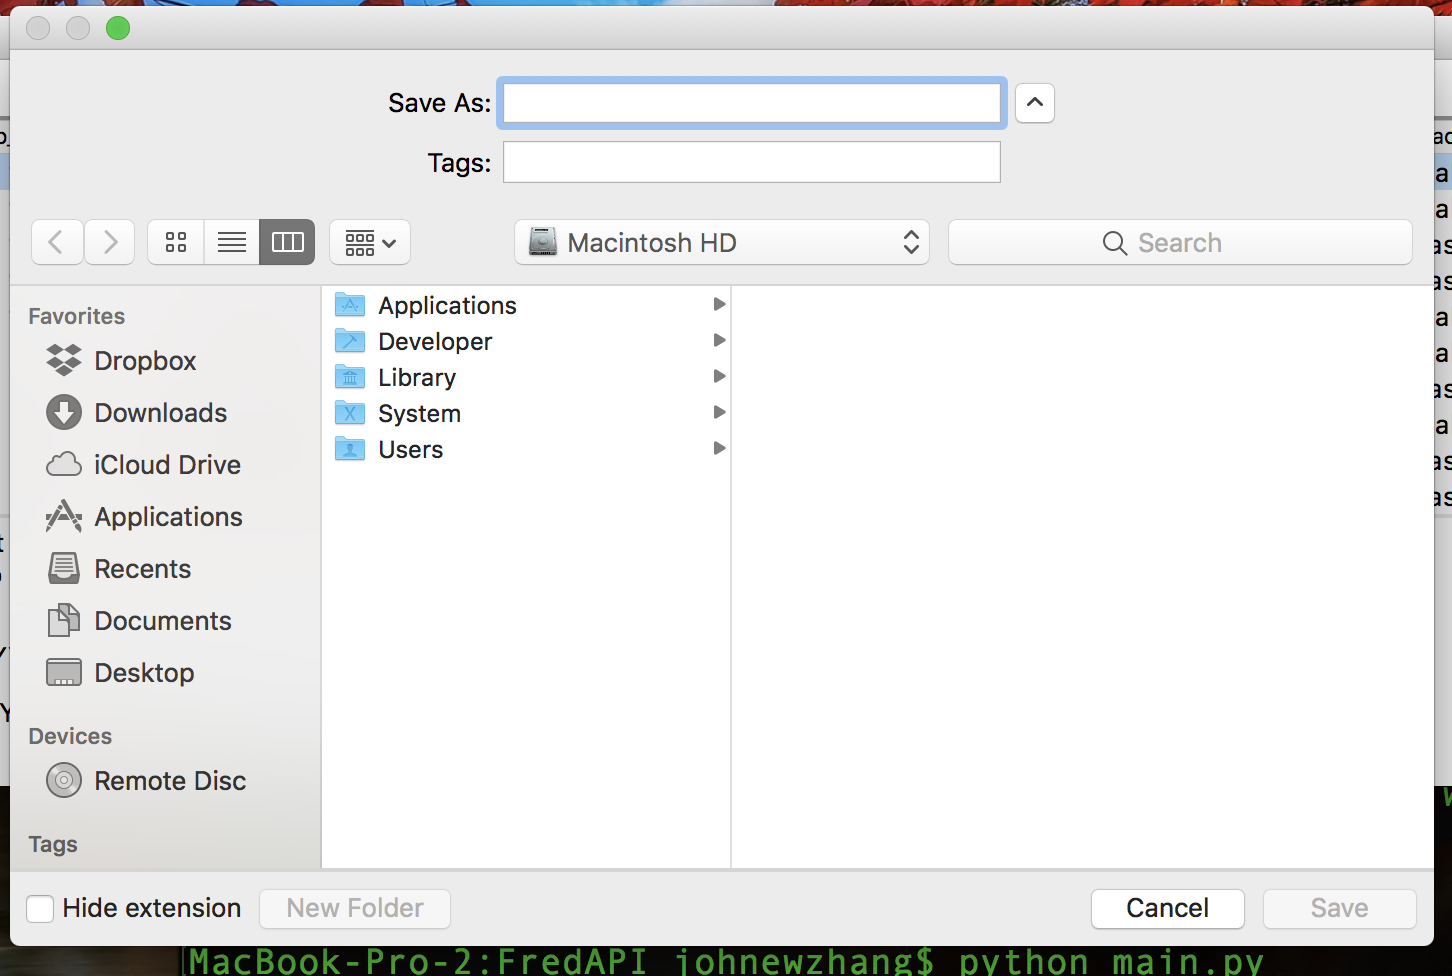
\includegraphics[width=0.5\linewidth]{img/save_as_page.png}
\caption{Save as Page}
\end{figure}



\section{Future Improvement}
\begin{itemize}
\item Include logging to trace any potential errors. 
\item Use a calendar to select data in the Start Date and End Date input sections. 
\item Add loading screen when querying and downloading data. 
\end{itemize}


%% The Appendices part is started with the command \appendix;
%% appendix sections are then done as normal sections
%% \appendix

%% \section{}
%% \label{}

%% References
%%
%% Following citation commands can be used in the body text:
%% Usage of \cite is as follows:
%%   \cite{key}          ==>>  [#]
%%   \cite[chap. 2]{key} ==>>  [#, chap. 2]
%%   \citet{key}         ==>>  Author [#]

%% References with bibTeX database:

\bibliographystyle{model1-num-names}
\bibliography{sample.bib}

%% Authors are advised to submit their bibtex database files. They are
%% requested to list a bibtex style file in the manuscript if they do
%% not want to use model1-num-names.bst.

%% References without bibTeX database:

% \begin{thebibliography}{00}

%% \bibitem must have the following form:
%%   \bibitem{key}...
%%

% \bibitem{}

% \end{thebibliography}


\end{document}

%%
%% End of file `elsarticle-template-1-num.tex'.